   \title{
The Hodgkin-Huxley neuron model V2.0
\iflatexml
\else
\vskip 1 cm
\small{The true physics and physiology behind neuronal operation}
\fi
}

\author{János Végh}
\date{\today}
\lxKeywords{dynamic neural modelling, Hodgkin-Huxley model, unified neuron model, neural information, neural computing, physics for biology, time-aware computing}
%============================================================
\begin{lxNavbar}

\includegraphics[width=0.375\textwidth]{../graphics/neurer.png}
The Hodgkin-Huxley neuron model V2.0\\
\small{The true physics and physiology\\behind neuronal operation}\\
(DANCES) Version \emph{\MyVersion}\\
%\@\today
\date{\today}
\lxContextTOC
%\\
%\href{../../simulator/ToIssue.html}{Report issue}
%\href{../manual.pdf}{Manual in .PDF form}
%\href{../../simulator/index.html}{Simulator}
%\href{../../simulator/ToCode.html}{Code}
%\href{../doxy/HTML/index.html}{Code documentation}
%\href{https://github.com/jvegh/Dynamic-Abstract-Neural-Computing/graphs/code-frequency}{Development pace}
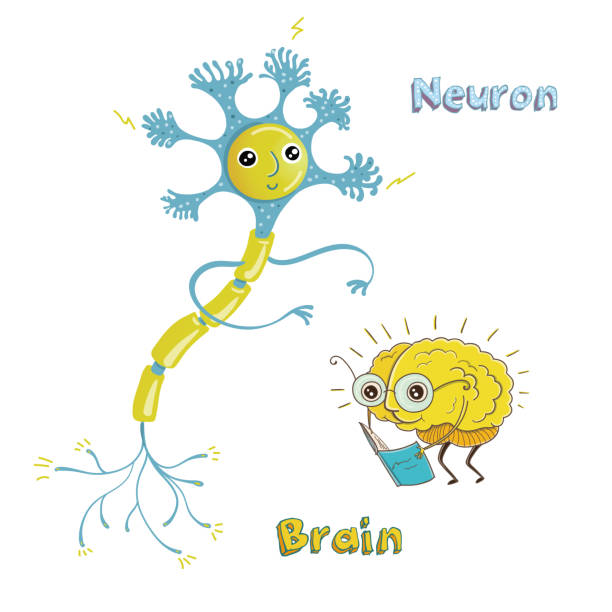
\includegraphics[width=0.41\textwidth]{../graphics/NeuronAndBrain.jpg}
\end{lxNavbar}

